\section{行事予定}
\begin{itemize}
\item 後期授業開始
10月1日(木)$\sim$
\item 第55回工大祭
11月21日(土)$\sim$11月22日(日)
\item トマトロボット競技会
12月18日$\sim$20日(金$\cdot$土$\cdot$日)
\end{itemize}

\section{現状}
\begin{itemize}
\item (9月7日)\\
アーム$\cdots$ハサミ。糸を巻き取ることで切断する.
機構$\cdots$仮にアームのものを作成することに決めた.
センサー$\cdots$キネクトもしくは、ステレオカメラを希望.
カメラとPSDセンサ(距離センサ)を使用する案もあります.
\item (9月8日)\\
3Dプリンターを利用してアームのモデルを作成しました。
\item (9月9日)\\
3Dプリンターを利用してハンドのモデルを作成しました。
切断実験に成功しました。\\
ハンドの概念機構はほぼ出来上がっているところまで進行している。よってこのまま釣り糸で切る方針でCAD設計に進行。アームはクレーン方式で進行。センサはKinectだけではできないかもしれない。台車とアームはRaspberry Piを用いる。Kinectの処理はPCを用いる。\\
プログラムに関しては、ROSを使用しない方針ですすめることに。カメラの情報をまだ扱えていないので、急ぎ達成すること。赤色と震度センサで認識をすることに決定。\\
git(arc)リポジトリを作成しました。
kinectのサンプルソースコードをgitにあげました。
\end{itemize}

\section{9月7日の西田先生との話し合いのまとめ}
部品の選定は以下のページを参考にすること
\begin{itemize}
\item ロボット王国
\item 共立エレショップ
\end{itemize}

当初の考えは、ボールねじを用いた超精密駆動が実現できるものであったが、たわみ等バランスを考えると、ネジが回らないとの指摘を受けました。

CADをして設計を早く完成させよう、という話でしたが、個人的な意見としては、もうCADをするよりも手で大まかに計算して作り始める方が良いのではないかと思います。

バランスのとれた設計とすること。
ゆっくり動くロボットを作ってもダメ。見ていて面白いものでなければいけない。
という内容でした。

\section{方針}
(9月7日)
\begin{itemize}
\item Raspberry Pi を使用して、土台を動かす
\item Raspberry Pi を使用して、アームを動かす
\item Kinect はPCに接続
\item PCがRaspberry Piに信号を送信する。
\item 計画が建てられない状況ですので、とりあえず今日はセンサを動かしてトマトを認識してみよう。
\end{itemize}

\par
(9月10日)
\begin{itemize}
\item 短期目標として、Kinect以外のセンサを手配すること、設計を早く終わらせることを目標にします。
\end{itemize}
\section{計画表}
計画として、軽く書いてみました。逐次更新します。

\begin{figure}[htbp]
\begin{center}
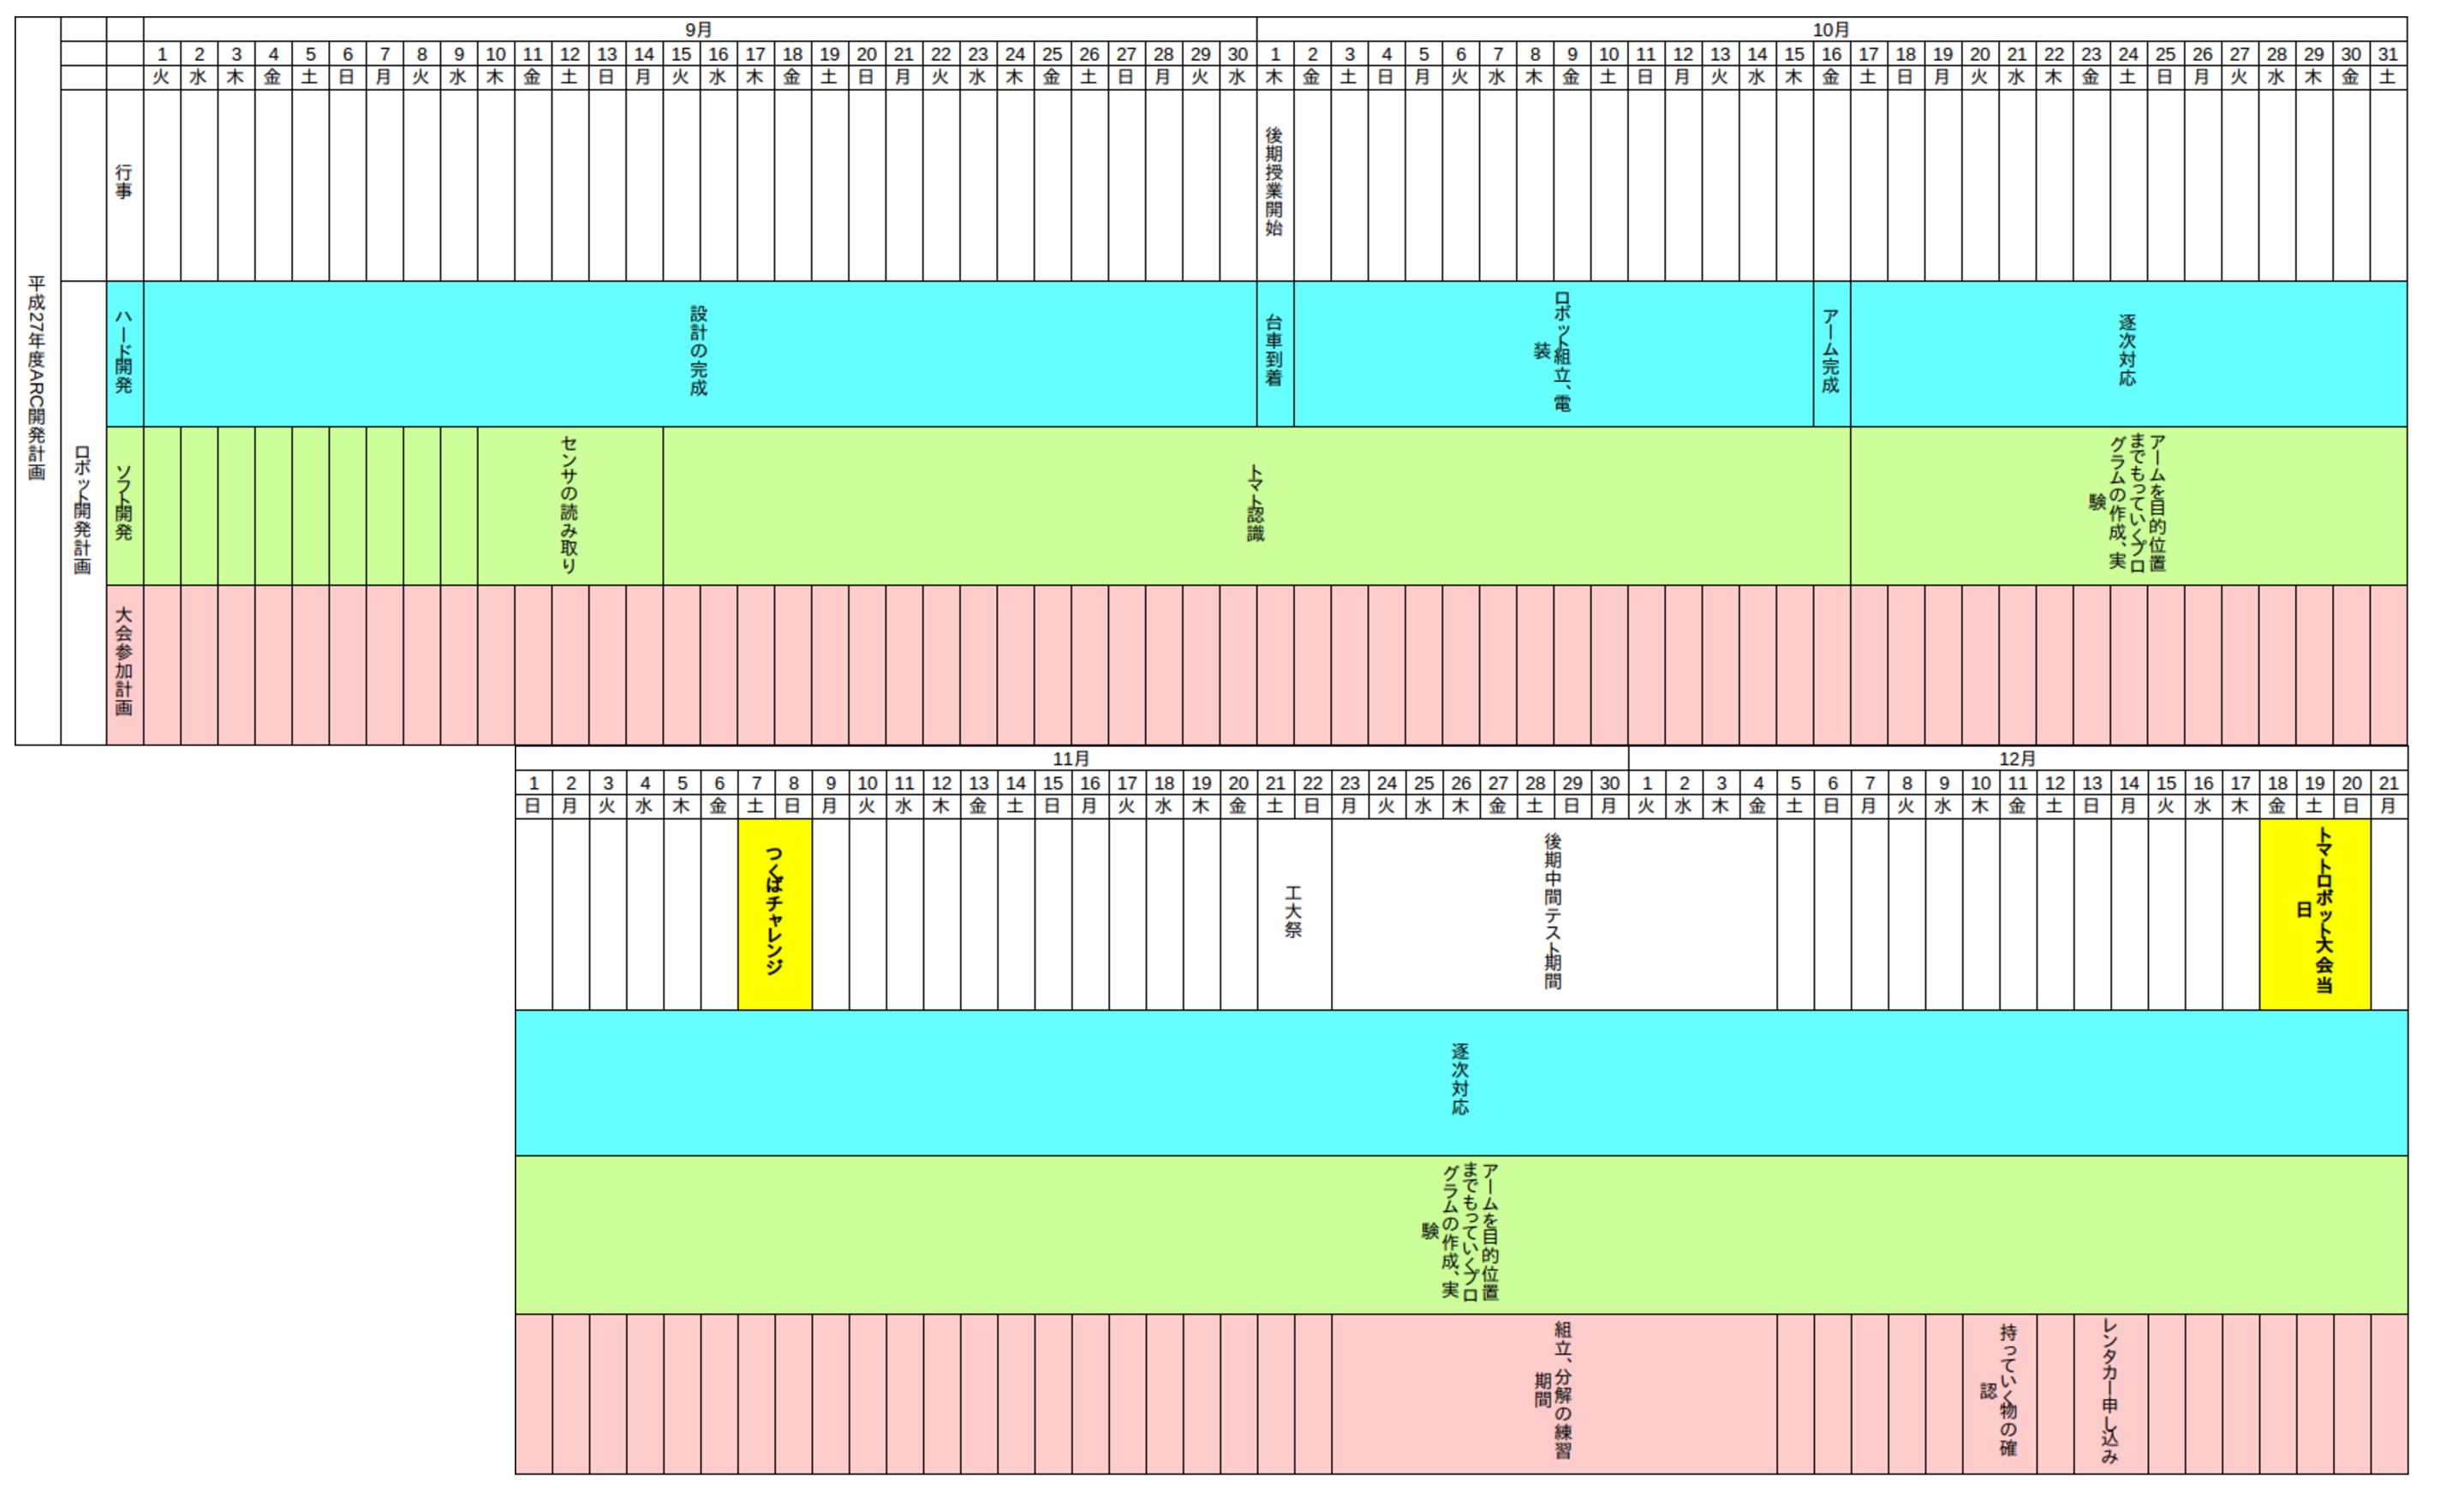
\includegraphics[width=25cm,angle=90]{../arc_plan.eps}
\end{center}
\caption{予定}
\end{figure}
